
\documentclass{article}
\usepackage{graphicx}
\usepackage{listings}
\usepackage{color}
\usepackage{amsmath}
\usepackage[margin=1in]{geometry}
\usepackage{caption}
\usepackage{float}
\usepackage{booktabs}
\usepackage{hyperref}
\hypersetup{colorlinks=true, linkcolor=blue, urlcolor=blue}

\definecolor{mygreen}{rgb}{0,0.6,0}
\definecolor{mygray}{rgb}{0.5,0.5,0.5}
\definecolor{mymauve}{rgb}{0.58,0,0.82}

\lstset{
  backgroundcolor=\color{white},
  basicstyle=\footnotesize\ttfamily,
  breaklines=true,
  captionpos=b,
  commentstyle=\color{mygreen},
  keywordstyle=\color{blue},
  stringstyle=\color{mymauve},
  numbers=left,
  numberstyle=\tiny\color{mygray},
  stepnumber=1,
  numbersep=5pt,
  showspaces=false,
  showstringspaces=false,
  showtabs=false,
  tabsize=2
}

\title{Lab Report: Regularization Techniques in Image Classification}
\author{Goutham Reddy Velma \\ Student ID: 12503589 \\ Advanced Programming \\ Instructor: Prof. Tobias Schaffer}
\date{\today}

\begin{document}

\maketitle

\begin{abstract}
The use of regularisation techniques in convolutional neural networks (CNNs) for the binary image classification task of differentiating between dogs and cats is examined in this report. To lessen overfitting and enhance generalisation, regularisation techniques like Dropout, L2 weight penalties, EarlyStopping, and Data Augmentation were investigated. TensorFlow was used to conduct experiments on the Dogs vs. Cats dataset, and models were assessed using confusion matrices, loss curves, and validation accuracy. While combination techniques showed difficulties, data augmentation produced the best validation performance. There is also discussion of suggestions for upcoming enhancements.
\end{abstract}

\section{Introduction}
The regularisation methods used on CNNs for the binary classification of the Dogs vs. Cats dataset are examined in this lab. To increase validation accuracy and generalisation, it emphasises techniques like Dropout, L2 regularisation, EarlyStopping, and Data Augmentation. Performance metrics, confusion matrices, and visual inspection of predictions are used to assess and compare various configurations.

\section{Methodology}

\subsection{Software and Hardware Used}
\begin{itemize}
    \item \textbf{Programming Language:} Python 3
    \item \textbf{Libraries:} TensorFlow, Keras, NumPy, Matplotlib, scikit-learn
    \item \textbf{Hardware:} Google Colab with NVIDIA T4 GPU
\end{itemize}

\subsection{Code Repository}
The full source code and results are hosted at:

\url{https://github.com/GouthamReddy-Velma/Regularization-Techniques-in-Image-Classification}

\subsection{Dataset Overview and Preprocessing}
The dataset used is the Kaggle Dogs vs. Cats dataset, which includes 25,000 RGB images equally divided between cats and dogs. Each image varies in resolution and background, necessitating preprocessing for standardization. The following steps were applied:

\begin{itemize}
    \item Images were resized to \textbf{150x150} pixels to ensure uniformity and reduce memory consumption, which also speeds up training without significantly affecting accuracy.
    \item Pixel values were scaled to the \textbf{[0,1]} range using \texttt{rescale=1./255} to normalize input features, improving model convergence.
    \item The dataset was split into \textbf{80\% training} (20,000 images) and \textbf{20\% validation} (5,000 images) to evaluate generalization on unseen data.
    \item Folder structure for Keras \texttt{flow\_from\_directory}:
    \begin{itemize}
        \item \texttt{train/cats}, \texttt{train/dogs}
        \item \texttt{validation/cats}, \texttt{validation/dogs}
    \end{itemize}
    \item The dataset is balanced with equal numbers of cat and dog images, helping prevent model bias towards either class.
\end{itemize}

\subsection{Data Augmentation Strategy}
To increase dataset variability and reduce overfitting, the following augmentations were applied on-the-fly to the training data:

\begin{itemize}
    \item Random horizontal flips, introducing mirror images to simulate different viewpoints.
    \item Small zoom range (0.2) to make the model robust to scale variations.
    \item Rotation up to 20 degrees to account for tilted images.
    \item Width and height shifts up to 20\% to simulate object displacement within the frame.
\end{itemize}

These augmentations were applied using Keras’s \texttt{ImageDataGenerator} API. Validation data was only rescaled, not augmented, to provide a consistent evaluation benchmark.

Data augmentation effectively increases the diversity of training examples without requiring additional labeled data, improving model generalization. However, it also increases training time due to on-the-fly transformations.

\subsection{Model Architecture}

All models were built using the \texttt{Sequential} API in Keras. Each architecture included:

\begin{itemize}
    \item Three convolutional blocks with increasing filters: 32, 64, 128
    \item \texttt{ReLU} activation after each convolution
    \item \texttt{MaxPooling2D} layers after each block
    \item A \texttt{Flatten} layer followed by a dense output head
    \item Binary classification output with \texttt{sigmoid} activation
\end{itemize}

Various regularization techniques were incorporated across models:
\begin{itemize}
    \item \textbf{Dropout:} Dropout layers with rates of 0.3 or 0.5 were applied after convolutional and/or dense layers.
    \item \textbf{L2 Regularization:} Kernel weight decay using \texttt{regularizers.l2(0.001)} was added to Conv2D and Dense layers.
    \item \textbf{Dropout + L2:} Combined model using both techniques simultaneously.
\end{itemize}

\newpage

The following diagram visually represents the CNN architecture described above. It illustrates the sequence of layers and operations involved in transforming an input image into a binary classification output. This helps in better understanding the model flow and where different regularization techniques were applied.

\vspace{1em}
\begin{center}
    \large\textbf{CNN Architecture Diagram}
\end{center}
\vspace{0.5em}

\begin{figure}[H]
\centering
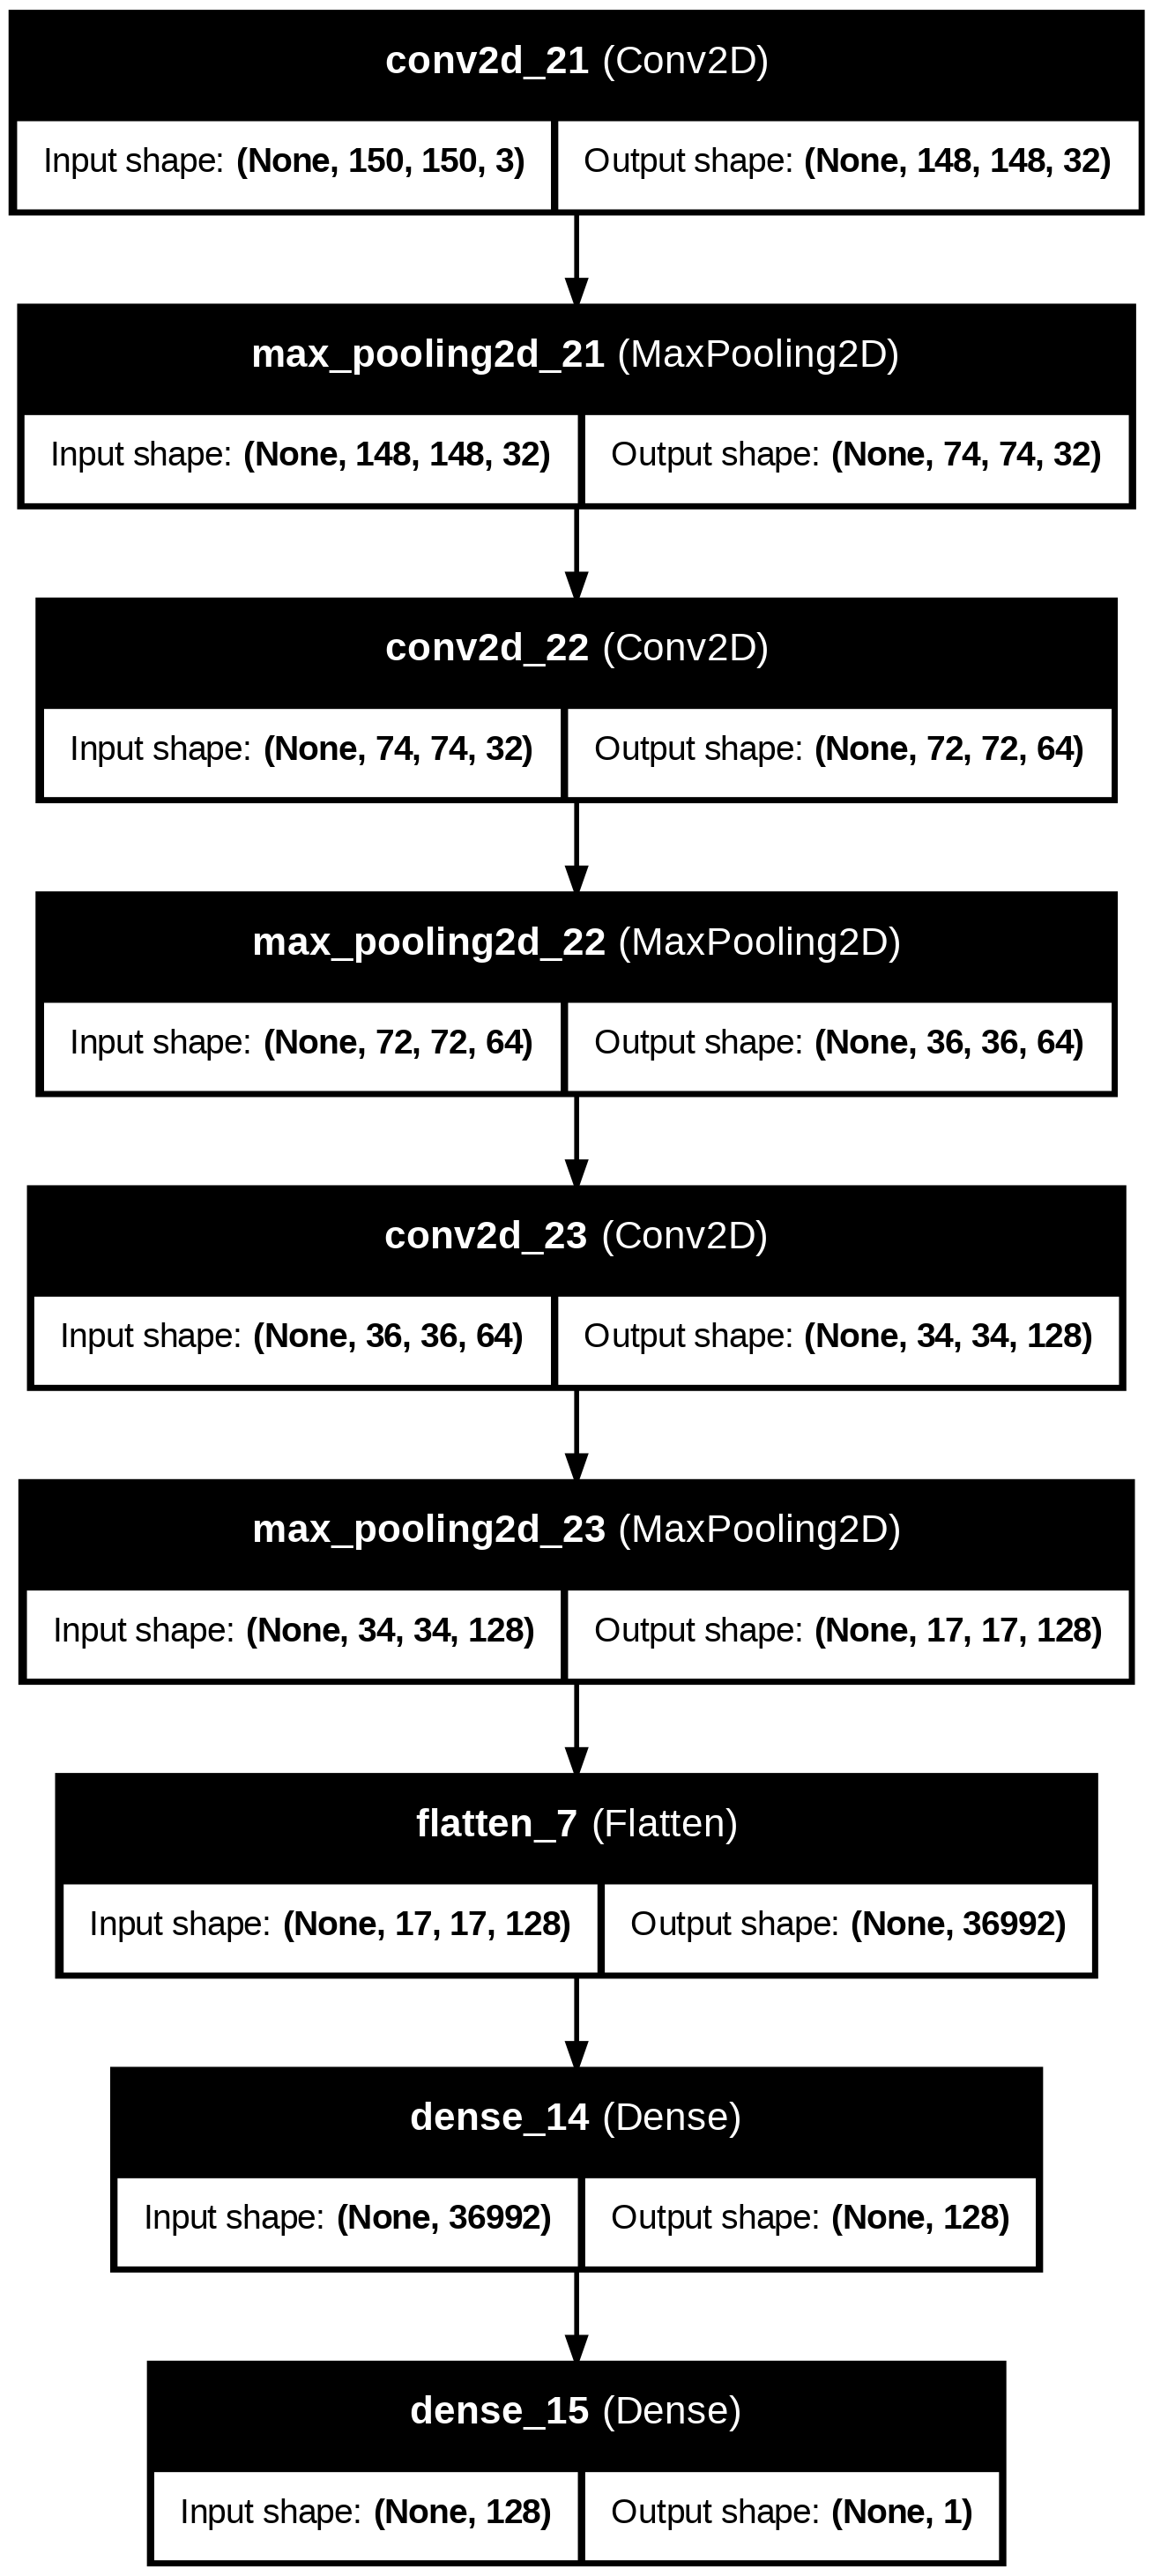
\includegraphics[width=0.5\linewidth]{cnn_diagram}
\caption{Architecture of the Convolutional Neural Network (CNN) used in the experiment}
\label{fig:cnn-architecture}
\end{figure}

\subsection{Training Configuration}
Each model was compiled and trained using the following settings:
\begin{itemize}
    \item \textbf{Loss Function:} Binary Crossentropy
    \item \textbf{Optimizer:} Adam (default learning rate)
    \item \textbf{Metrics:} Accuracy
    \item \textbf{Batch Size:} 32
    \item \textbf{Epochs:} Up to 20
\end{itemize}

\subsection{Callbacks and Monitoring}
An \texttt{EarlyStopping} callback was used to prevent overfitting by monitoring the validation loss. It was configured with:
\begin{itemize}
    \item \textbf{Monitor:} \texttt{val\_loss}
    \item \textbf{Patience:} 3 epochs
    \item \textbf{Mode:} \texttt{min}
\end{itemize}

Additionally, training histories (accuracy and loss) were saved and visualized for each run to compare learning dynamics.

\subsection{Evaluation Tools}
Post-training evaluation included:
\begin{itemize}
    \item Confusion Matrix (via \texttt{sklearn.metrics.confusion\_matrix})
    \item Classification Report (Precision, Recall, F1-score)
    \item Visual inspection of misclassified images
    \item Performance plots for training vs. validation loss/accuracy
\end{itemize}

\subsection{Code Implementation}

\subsubsection*{Data Augmentation}
\begin{lstlisting}[language=Python]
train_datagen = ImageDataGenerator(
    rescale=1./255,
    rotation_range=20,
    width_shift_range=0.2,
    height_shift_range=0.2,
    horizontal_flip=True,
    zoom_range=0.2
)
\end{lstlisting}

\subsubsection*{L2 Regularization}
\begin{lstlisting}[language=Python]
Conv2D(64, (3, 3), activation='relu', 
        kernel_regularizer=regularizers.l2(0.001))
\end{lstlisting}

\subsubsection*{Dropout}
\begin{lstlisting}[language=Python]
Dropout(0.3)
\end{lstlisting}

\subsubsection*{Baseline Model}
\begin{lstlisting}[language=Python]
model_basic = Sequential([
    Conv2D(32, (3, 3), activation='relu'),
    MaxPooling2D(2, 2),
    Conv2D(64, (3, 3), activation='relu'),
    MaxPooling2D(2, 2),
    Conv2D(128, (3, 3), activation='relu'),
    MaxPooling2D(2, 2),
    Flatten(),
    Dense(128, activation='relu'),
    Dense(1, activation='sigmoid')
])
\end{lstlisting}

\subsubsection*{Dropout + L2}
\begin{lstlisting}[language=Python]
model_combo = Sequential([
    Conv2D(32, (3, 3), activation='relu', kernel_regularizer=l2(0.001)),
    MaxPooling2D(2, 2),
    Dropout(0.3),
    Conv2D(64, (3, 3), activation='relu', kernel_regularizer=l2(0.001)),
    MaxPooling2D(2, 2),
    Dropout(0.3),
    Conv2D(128, (3, 3), activation='relu', kernel_regularizer=l2(0.001)),
    MaxPooling2D(2, 2),
    Dropout(0.3),
    Flatten(),
    Dense(128, activation='relu', kernel_regularizer=l2(0.001)),
    Dropout(0.5),
    Dense(1, activation='sigmoid')
])
\end{lstlisting}

\subsubsection*{EarlyStopping}
\begin{lstlisting}[language=Python]
early_stop = EarlyStopping(monitor='val_loss', patience=3)

model.fit(train_generator,
          validation_data=val_generator,
          epochs=20,
          callbacks=[early_stop])
\end{lstlisting}

\section{Results}

\subsection*{Accuracy and Loss Graphs}
Performance of various models across epochs is shown below:

\paragraph{Baseline Model Accuracy and Loss}
The baseline model shows steady improvement in training accuracy with a corresponding decrease in loss. However, validation accuracy plateaus earlier, indicating potential overfitting beginning after around 10 epochs.

\begin{figure}[H]
\centering
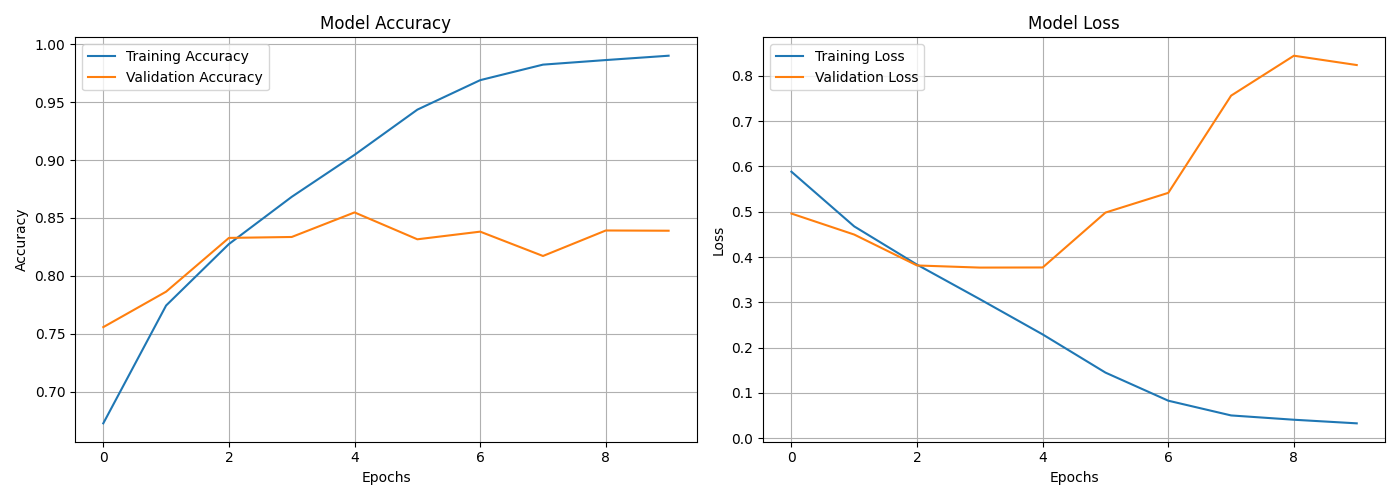
\includegraphics[width=0.9\linewidth]{baseline_accuracy_loss.png}
\caption{Baseline Model Accuracy and Loss}
\end{figure}

\paragraph{Dropout Regularization}
Applying Dropout slightly improves validation accuracy by reducing overfitting. The loss curves are smoother and the gap between training and validation metrics narrows compared to the baseline.

\begin{figure}[H]
\centering
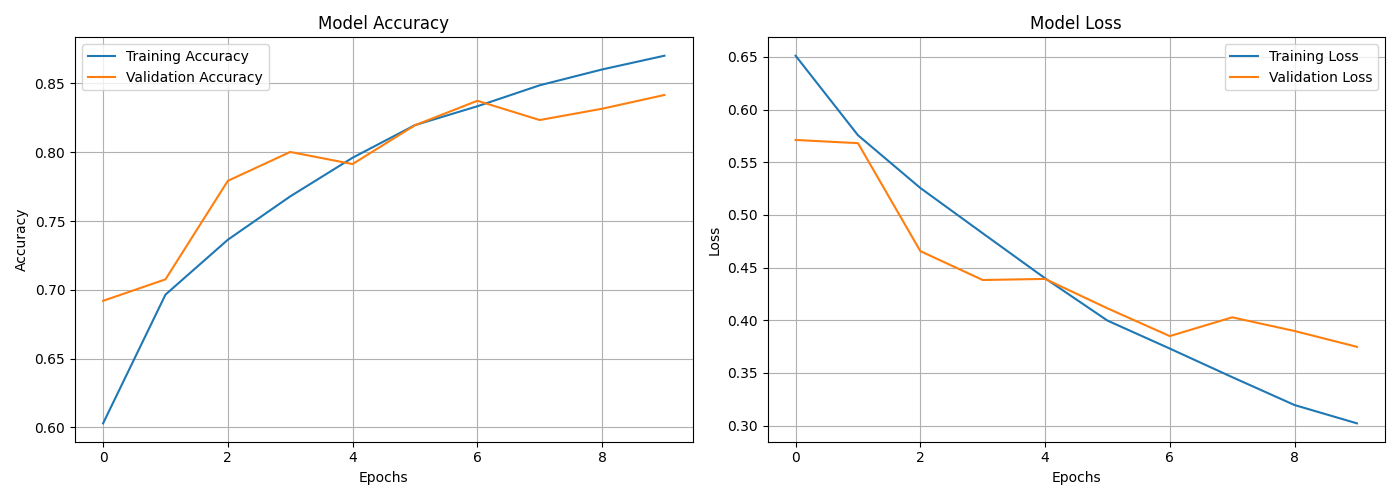
\includegraphics[width=0.9\linewidth]{dropout_accuracy_loss.png}
\caption{Dropout Regularization}
\end{figure}

\paragraph{L2 Regularization}
L2 regularization introduces weight decay that penalizes large weights. This results in more generalizable models as seen by slightly better validation accuracy and more stable loss reduction.

\begin{figure}[H]
\centering
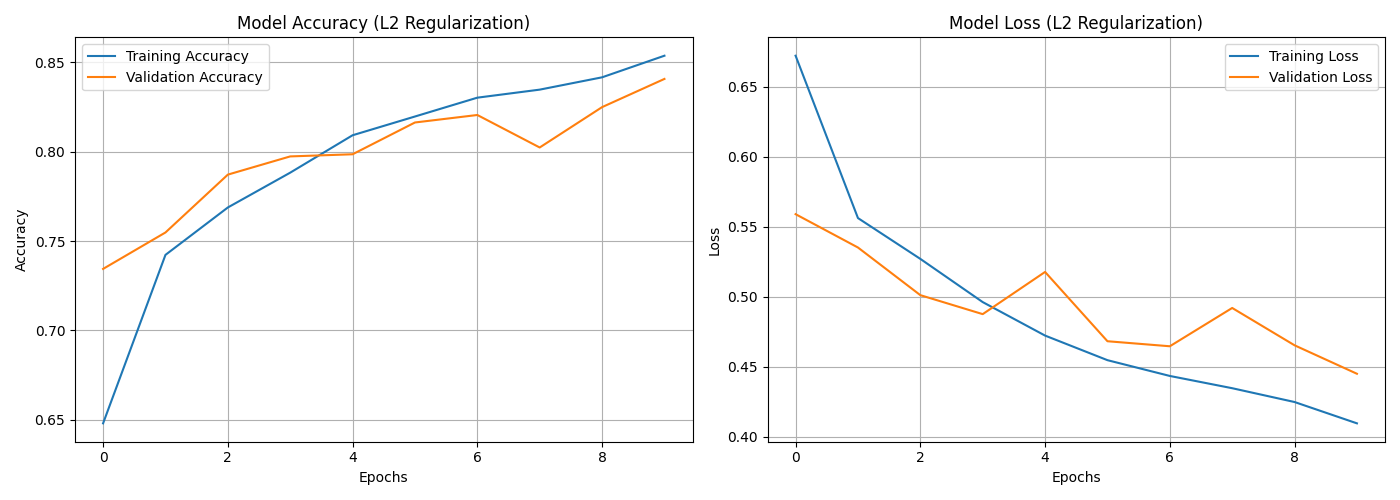
\includegraphics[width=0.9\linewidth]{l2_accuracy_loss.png}
\caption{L2 Regularization}
\end{figure}

\paragraph{Dropout + L2 (Combined)}
Combining Dropout and L2 surprisingly led to poorer validation performance and unstable training curves, likely due to over-regularization causing underfitting.

\begin{figure}[H]
\centering
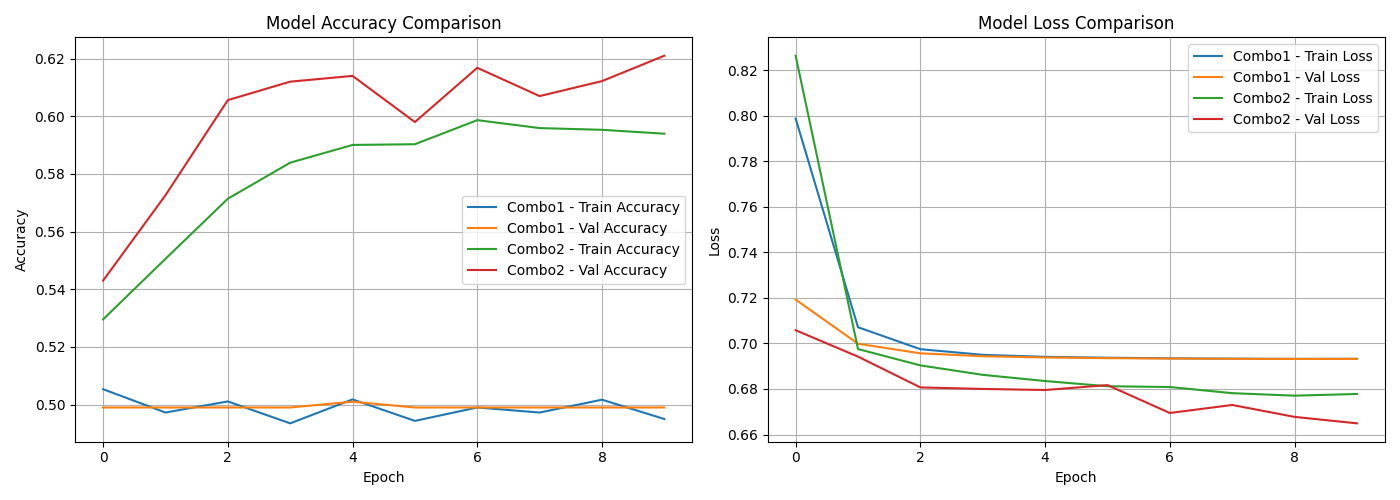
\includegraphics[width=0.9\linewidth]{combo_accuracy_loss.png}
\caption{Dropout + L2 (Combined)}
\end{figure}

\paragraph{Model with EarlyStopping}
EarlyStopping halts training once validation loss stops improving, preventing overfitting. This is evident by earlier convergence around 7 epochs without loss spikes.

\begin{figure}[H]
\centering
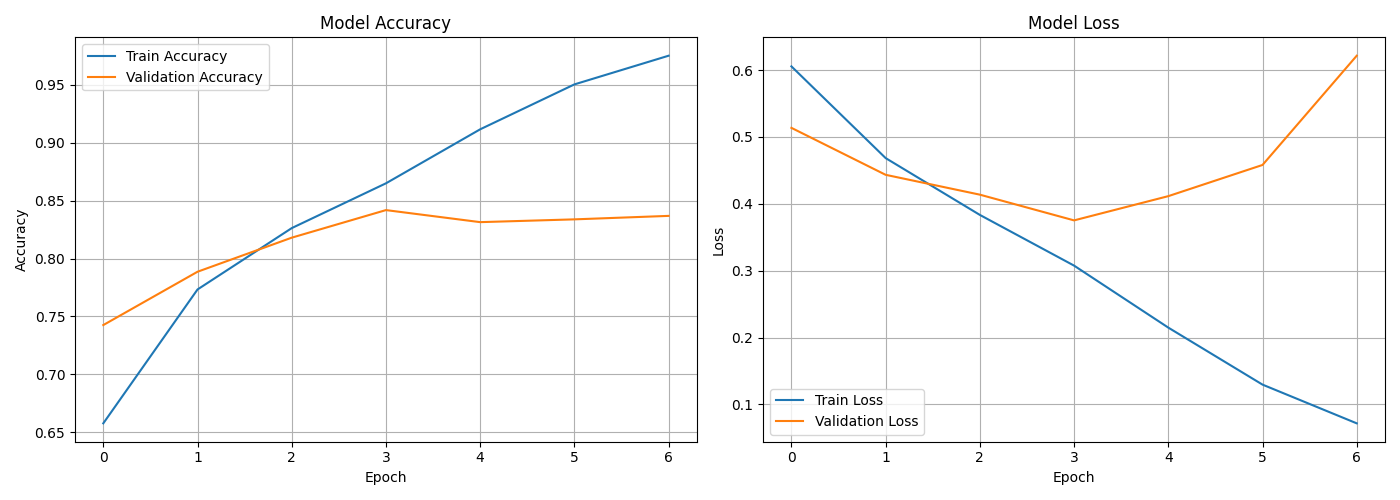
\includegraphics[width=0.9\linewidth]{earlystopping_accuracy_loss.png}
\caption{Model with EarlyStopping}
\end{figure}

\paragraph{Data Augmentation}
Data augmentation significantly improves validation accuracy by increasing data diversity. The model shows more consistent learning with reduced overfitting, as training and validation curves remain closer throughout.

\begin{figure}[H]
\centering
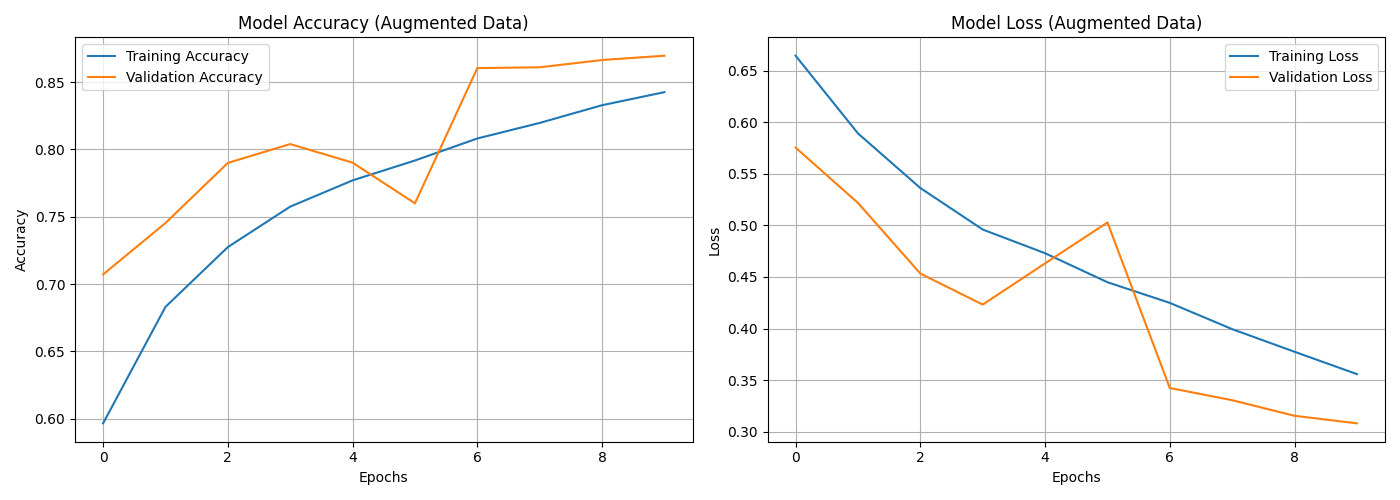
\includegraphics[width=0.9\linewidth]{augmentation_accuracy_loss.png}
\caption{Data Augmentation}
\end{figure}

\subsection*{Summary Table}

\begin{table}[H]
\centering
\begin{tabular}{|l|c|c|c|}
\hline
\textbf{Technique} & \textbf{Augmentation} & \textbf{Val Accuracy} & \textbf{Epochs to Converge} \\
\hline
Baseline & No & 83.90\% & 10 \\
Dropout (0.3/0.5) & No & 84.16\% & 10 \\
L2 (0.001) & No & 84.08\% & 10 \\
Dropout + L2 (Combo) & No & 49.9\%, 62.1\% & 10 \\
EarlyStopping & No & 83.68\% & 7 \\
\textbf{Data Augmentation} & \textbf{Yes} & \textbf{86.96\%} & \textbf{10} \\
\hline
\end{tabular}
\caption{Comparison of Techniques and Their Performance}
\end{table}

\subsection*{Confusion Matrix}
\begin{figure}[H]
\centering
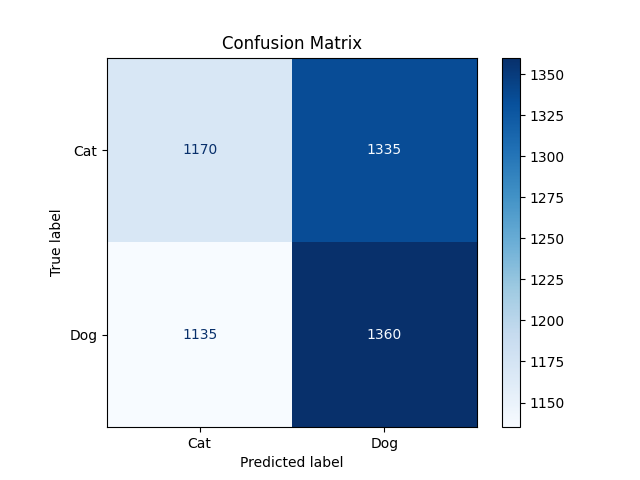
\includegraphics[width=0.6\linewidth]{confusion_matrix.png}
\caption{Confusion Matrix of Final Model}
\end{figure}

\subsection*{Confusion Matrix (Table Format)}

\noindent
\textbf{Note:} \\
\textbf{TN (True Negative):} Correctly predicted cats \\
\textbf{FP (False Positive):} Cats incorrectly predicted as dogs \\
\textbf{FN (False Negative):} Dogs incorrectly predicted as cats \\
\textbf{TP (True Positive):} Correctly predicted dogs

\begin{table}[H]
\centering
\begin{tabular}{|l|c|c|}
\hline
\textbf{Actual / Predicted} & \textbf{Cat (0)} & \textbf{Dog (1)} \\
\hline
\textbf{Cat (0)} & 1170 (TN) & 1335 (FP) \\
\hline
\textbf{Dog (1)} & 1135 (FN) & 1360 (TP) \\
\hline
\end{tabular}
\caption{Confusion Matrix showing model performance on validation data}
\end{table}

The confusion matrix indicates how well the model distinguishes cats and dogs. It reveals true positives, false positives, true negatives, and false negatives — essential for error analysis.

\subsection*{Misclassified Samples}
\begin{figure}[H]
\centering
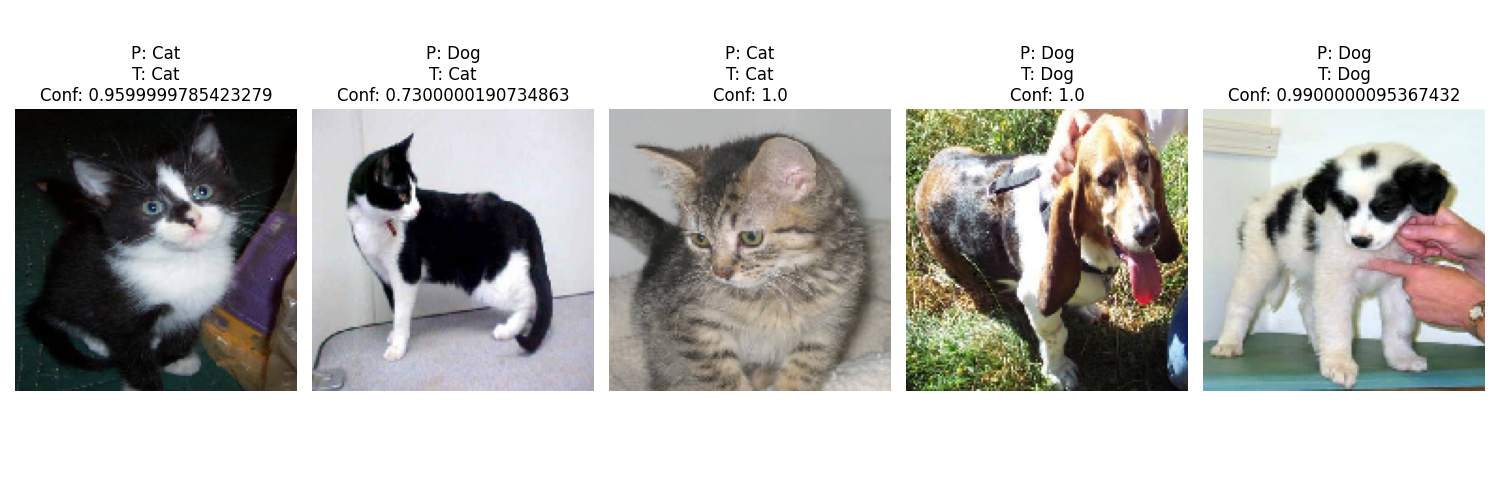
\includegraphics[width=0.9\linewidth]{misclassified_samples.png}
\caption{Misclassified Images with Predictions}
\end{figure}

The misclassified images show cases where the model failed. These may include difficult angles, poor lighting, or class ambiguity, and help identify where the model can improve.

\section{Challenges, Limitations, and Error Analysis}

\subsection{Challenges}
\begin{itemize}
    \item Organizing the dataset and understanding augmentation parameters.
    \item Properly combining Dropout with L2 without underfitting.
\end{itemize}

\subsection{Error Analysis}
\begin{itemize}
    \item Confusion occurred in complex or noisy images.
    \item Augmentation helped generalization but sometimes slowed training.
\end{itemize}

\subsection{Limitations}
\begin{itemize}
    \item Basic CNNs have limited accuracy without transfer learning.
    \item Misclassification on similar-looking animals remains a challenge.
\end{itemize}

\section{Discussion}
Both L2 and Dropout enhanced generalisation. Regularisation was probably too strong, which is why their combination didn't produce the best results. Training time was decreased thanks to EarlyStopping. Performance was greatly improved by augmentation, making it the optimal setup all around.

\section{Conclusion}
The significance of regularisation in enhancing CNN generalisation was reaffirmed by this lab. The use of data augmentation produced the best results. All things considered, the experiment showed how deep learning models could be practically adjusted for actual image classification.

\section*{References}
\begin{itemize}
    \item F. Chollet, “Deep Learning with Python”, Manning, 2017.
    \item TensorFlow Docs: \url{https://www.tensorflow.org/}
    \item Kaggle Cats vs. Dogs: \url{https://www.kaggle.com/c/dogs-vs-cats}
\end{itemize}

\end{document}
